\documentclass[../main.tex]{subfiles}
\begin{document}

\subsection{Introduction} Limits are a way of skirting the normal rules of math. Without the knowledge of limits, whenever a function divides by 0 or involves $\infty$ in any way, calculations become impossible. Limits take the rules of math a little less seriously and can be used to calculate what a value ``should be''. A simple example of where limits come in handy is when there is a ``hole'' in a graph:
\begin{center}
\begin{tikzpicture}
	\begin{axis}
	\addplot[domain=0:4,blue]{x+2};
	\addplot[holdot] coordinates{(2,4)};
	\end{axis}
\end{tikzpicture}
\end{center}
$$f(x)=\frac{x^2-4}{x-2}$$
Because $f(x)$ divides by 0 when $x=2$, there can be no answer here. However, we can tell that $f(2)$ should be 4 ignoring the division by zero. We can tell this because as $x$ becomes greater and nearer to 2 (approaching $x=2$ from the left), the value of $f(x)$ approaches 4. Similarly, when $x$ decreases and becomes nearer to $x=2$ (approaching $x=2$ from the right), the value of $f(x)$ approaches 4. Therefore, as both sides of $x=2$ become closer and closer, they converge upon a single point: $f(2)=4$.
\subsection{Limits} Limits can help us with the preceding problem. A limit returns the value of a function that it should be. \textit{We define the limit to be equal to the point both sides of a graph approaches.} A simple way to write this is $\lim\limits_{x\to c^{+}}f(x)$ to represent the limit as $x$ increases to the value $c$ and $\lim\limits_{x\to c^{-}}f(x)$ to represent the limit as $x$ decreases to the value $c$. In other words, $\lim\limits_{x\to c^{+}}f(x)$ is the value we approach moving to the right towards $c$ and $\lim\limits_{x\to c^{-}}f(x)$ is the value we approach moving to the left towards $c$. We define $$\lim\limits_{x\to c} f(x)= \lim\limits_{x\to c^{+}} f(x)=\lim\limits_{x\to c^{-}}f(x)$$ If the limits moving to the left and moving to the right are not equal, the statement above is false and we say that the limit does not exist. For example, the limit as $x$ approaches 2 in this graph doesn't exist:
\begin{center}
	\begin{tikzpicture}
	\begin{axis}
	[
	domain=-2:6, restrict y to domain=-4:4,
	]
	\addplot[domain=-2:6,red,samples=50]{1/(x-2)};
	\end{axis}
	\end{tikzpicture}
\end{center}
\subsection{Applications of Limits} Limits are very useful when needing to find a value that shouldn't necessarily exist. We can use limits to calculate holes in graphs from what we saw earlier, but we can also use them to approach unapproachable values like $\infty$. As we can only approach $\infty$ from one side, we write the limit as $\lim\limits_{x\to\infty} f(x)$ for positive $\infty$ and $\lim\limits_{x\to\ -\infty} f(x)$ for $-\infty$.
\subsection{Calculating limits} Unfortunately, there's no simple and easy way to calculate limits. The simplest way is just to ``plug in'' to the function but at some points like holes in the graph or $\infty$, we don't have that luxury. Instead, we can reduce or rewrite equations and also apply some general common sense. For example, $\lim\limits_{x\to\infty} \frac{1}{x}$ must be 0 because as $x$ gets larger, $\frac{1}{x}$ gets smaller to some point at which it must be 0. Using reduction and logic, we may progress on to more complex ideas involving limits where direct substitution fails.
\paragraph{``Plugging In''} In the end, all limit problems will need to have their value inserted at some time. For example, the limit $\lim\limits_{x\to 0} x^2+1=1$. No tricks here, plugging in 0 does return 1. We do not have to deal with any division by zero or infinities, so there is no need to manipulate the problem.
\paragraph{Reduction} Reduction is relatively simple. If we go back to our example of $$f(x)=\frac{x^2-4}{x-2}$$ we can see that this problem can factor into $$f(x)=\frac{(x-2)(x+2)}{x-2}$$ which cancels and gives us $$f(x)=x+2$$We now see that there does exist a limit at $x=2$, $f(2)=2+2=4$ Previously, directly plugging in 2 would not return a real value.
\paragraph{Sense at $\infty$} $\infty$ is a hard concept to grasp and work with in mathematics. Limits can make this easier because while we cannot \textit{directly compute} $\infty$, we can approximate it exactly. For example, in the case of $f(x)=\frac{1}{x^2}$, we see that the limit at $\infty$ must be zero. As $x$ increases, $f(x)$ drops ever closer to 0:$$f(10)=0.01$$$$f(100)=0.0001$$$$f(1000)=0.000001$$$$etc.$$ Similarly, as $x$ approaches $\infty$, $$g(x)=\frac{3x}{4x+1}$$ approaches $\frac{3}{4}$: $$g(10)=\frac{30}{41}$$$$g(100)=\frac{300}{401}$$$$g(1000)=\frac{3000}{4001}$$$$etc.$$
\subsection{When Limits Don't Exist} Limits don't exist when:
\begin{enumerate}
\item $\lim\limits_{x\to c^+} \neq \lim\limits_{x\to c^-}$
\begin{center}
\begin{tikzpicture}
	\begin{axis}
	\addplot[domain=-1:0,blue,samples=50]{x^2+1};
	\addplot[domain=0:1, blue]{-.25*x+0.75};
	\addplot[holdot] coordinates{(0,1)};
	\addplot[dot] coordinates{(0,.75)};
	\end{axis}
\end{tikzpicture}
$$\lim_{x\to 0} f(x) \text{ Does Not Exist}$$
\end{center} 
\par The reason why the limit cannot exist at 0 here is that when $f(x)$ approaches 0 from the right side ($0^-$), the limit is 1. As $f(x)$ approaches 0 from the left side ($0^+$), the limit is 0.75. The limit is one point and because $0.75\neq 1$, there is no solution. We say that the limit \textit{diverges}.
\newpage
\item The graph oscillates uncontrollably:
\begin{center}
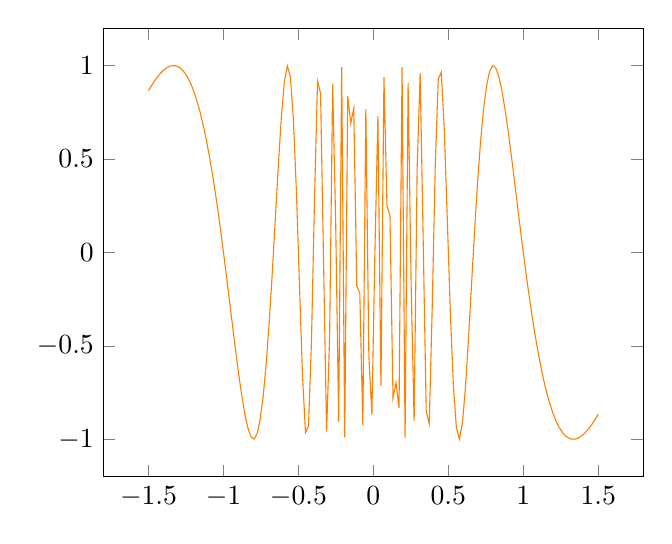
\begin{tikzpicture}
	\begin{axis}
	\addplot[domain=-1.5:1.5,orange,samples=150]{sin(360*(x)^-1)};
	\end{axis}
\end{tikzpicture}
$$\lim_{x\to 0} \text{sin} \left ( \frac{1}{x} \right ) \text{ Does Not Exist}$$
\end{center} \par The graphing utility doesn't even have any idea what's going on. We can't blame it because the graph starts oscillating faster and faster closer to 0. There is no point the graph can approach. Therefore, the limit must not exist here.
\newpage
\item The graph oscillates at $\infty$
\begin{center}
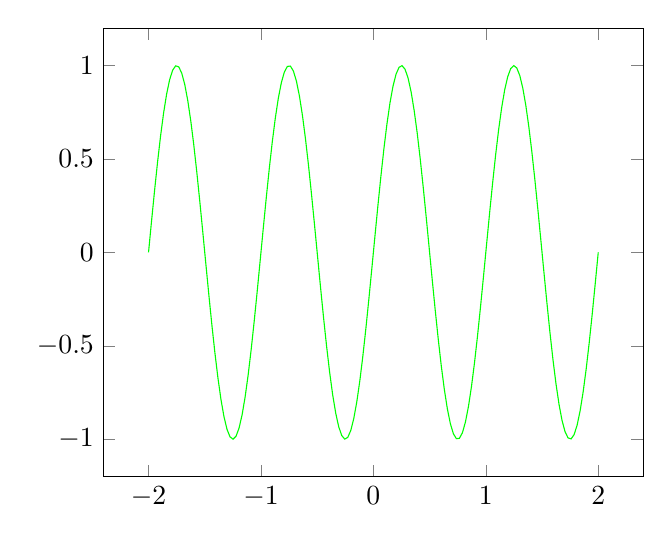
\begin{tikzpicture}
	\begin{axis}
	\addplot[domain=-2:2,green,samples=150]{sin(360*x};
	\end{axis}
\end{tikzpicture}
$$\lim_{x\to\infty} \text{sin}(x) \text{ Does Not Exist}$$
\end{center}
\par Is $\infty$ an integer? Or where does it fall exactly? If you define $\infty$ to be a value, something can always be added to that value. Therefore, there is no single value that this graph will approach. In fact, it will approach all numbers in the interval [-1,1]. For a periodic graph like sin($x$), there can be no limit because the graph will never stop oscillating.
\end{enumerate}
\end{document}